\section{Android系统架构}
Android系统由多个软件层次构成, 这些层次功能分明, 每一层都对其上的一层提供服务, 构成一个5层的软件栈\juhao 软件栈最底层为Linux内核层, 其上为硬件抽象层, 之后为本地函数库层, 该层次包括了Android Runtime和其他的一些本地函数库, 再上层为Android框架层, 该层包括了提供给应用程序的API和系统管理服务程序, 最上层为应用层, 该层次为用户直接交互的应用程序运行的层次\juhao  图\ref{androidStructure}给出了各层次的组件和关系\juhao
\begin{figure}[ht]
\centering
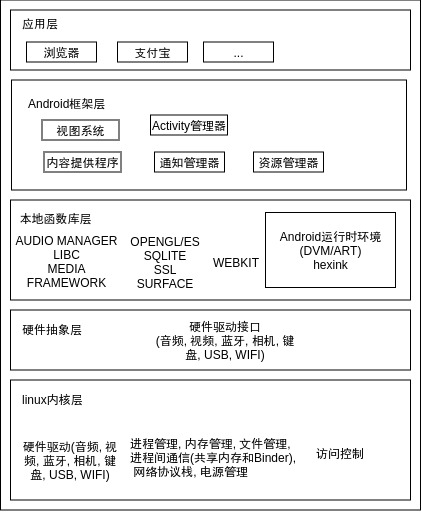
\includegraphics[width=9cm]{android_structure.jpg}
\caption{Android系统架构}
\label{androidStructure}
\end{figure}

\subsection*{Linux内核层} 
Android基于修改的Linux内核构建, Linux内核为Android系统提供了操作系统的基本功能, 包括进程管理, 内存管理, 文件管理, 进程间通信(共享内存和Binder), 网络协议栈, 电源管理, 许多设备驱动程序(音频, 视频, 蓝牙, 相机, 键盘, USB, WIFI等)以及访问控制机制(基于用户和用户组的访问控制和selinux)\juhao 这些功能通过系统调用的方式提供给上层使用, 因此, 监控系统调用的使用情况能够获取到应用对关键资源的访问行为\juhao

\subsection*{硬件抽象层}
硬件抽象层是定义了用于更高层次调用对应硬件驱动的接口, 屏蔽了不同厂商的同种设备驱动的差异, 降低Android系统与硬件的耦合度, 便于Android系统的移植\juhao 硬件抽象层包含多个库模块,其中每个模块都为特定类型的硬件组件实现一个接口,例如相机或蓝牙模块。当更高层次要求访问设备硬件时,Android系统将为该硬件组件加载库模块。

\subsection*{本地库层}
本地库层由许多由C/C++开发的系统运行库组成\juhao 这些运行库主要分为两部分, 第一分部为Android运行时环境相关的库, 第二部分为其他系统运行库\juhao 

Android运行时环境由给应用提供Java运行环境的虚拟机实现和实现Java API的核心运行时库组成\juhao 虚拟机实现在Android4.4之前为Dalvik虚拟机, Android4.4时Android Runtime(ART)虚拟机作为实验特性加入, 并和Dalvik虚拟机共存, Android5.0之后只保留了ART虚拟机\juhao Android框架层的许多服务程序和应用层的应用软件就运行在自身的虚拟机实例中\juhao 核心运行时库提供了Java语言的大部分标准API\juhao

其他系统运行库包括许多重要的功能的实现, 主要包括以下部分: 
AUDIO MANAGER用于管理音频输入输出; 
LIBC提供了C语言标准函数库; 
MEDIA FRAMEWORK提供了对常见音频和视频处理的支持; 
OPENGL/ES提供了2D/3D图形绘制功能;
SQLITE提供了访问SQLite数据库的函数;
SSL提供了常见的加密功能;
SURFACE MANAGER提供对显示子系统的支持和管理;
WEBKIT提供了浏览器引擎的实现\juhao

本地库层的各种功能函数除了提供给Android系统自身以实现系统服务功能, 还可以通过Android Native Development Kit(NDK)让应用程序通过Java Native Interface(JNI)调用, 因此对本层函数调用情况的监控可以获取到应用的行为\juhao

\subsection*{Android框架层}
Android框架层包括了许多系统服务程序和组件以及提供给应用程序的访问系统资源的Java API\juhao 这些服务程序和组件主要包括以下几部分:

1. 资源管理器,用于访问非代码资源,例如本地化的字符串、图形和布局文件

2. 通知管理器,可让所有应用在状态栏中显示自定义提醒

3. Activity管理器,用于管理应用的生命周期,提供常见的导航返回栈

4. 内容提供程序,可让应用访问其他应用(例如“联系人”应用)中的数据或者共享其自己的数据

5. 丰富、可扩展的视图系统,可用以构建应用的 UI,包括列表、网格、文本框、按钮甚至可嵌入的网络浏览器

Android框架层是与应用程序联系最紧密的层次, 也是应用程序最容易访问系统资源的层次, 因此对该层次提供的API的监控能够显示应用的主要行为\juhao

\subsection*{应用层}
应用层包括了所有用户直接使用的应用软件,例如电话、短信、浏览器、微信、支付宝等\juhao 这些应用软件主要由Java语言开发, 通过调用Android框架层提供的API和Java语言的标准API实现功能, 每个应用运行于自己独立进程中的虚拟机实例中, 多个应用间借助框架层提供的API通信(进程间通信最终由内核实现)\juhao 利用NDK, 应用也可以实现自己的本地库, 访问Android系统本地库层的开放甚至隐藏的函数, 并通过JNI在应用的Java部分调用自身的本地库中的本地函数\juhao 由于应用能够直接执行本地代码, 增加了应用程序行为涉及的层次, 需要同时在Java层次和本地层次监控应用的执行才能获取到应用的所有行为\juhao


\section{Android应用结构}
\subsection{应用安装包结构}
Android应用程序主要以Android Package(APK)的文件形式分发和安装\juhao APK文件本质上是一种zip压缩文件, 由多个文件和文件夹组成 其中包含了应用的代码文件、资源文件、证书文件和清单文件, 以apk作为文件后缀名\juhao 图\ref{packageStructure}给出了APK文件的内部结构\juhao
\begin{figure}[ht]
	\centering
	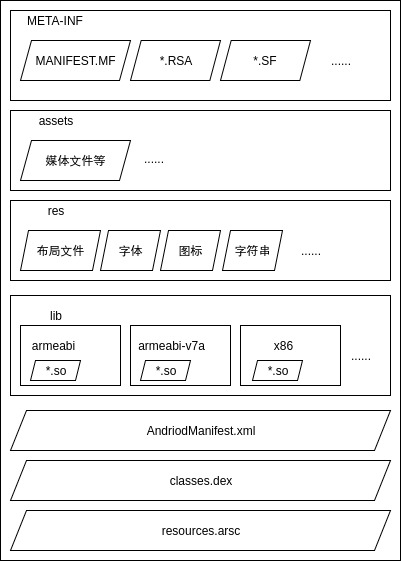
\includegraphics[width=8cm]{package_structure.jpg}
	\caption{APK文件结构}
	\label{packageStructure}
\end{figure}

META-INF文件夹包含了与APK文件的签名和校验相关的文件, 一般应该包括至少3个文件:MANIFEST.MF、*.RSA、*.SF(“*”表示文件名不确定)\juhao 
其中MANIFEST.MF记录了APK中的所有文件名和经过base64编码的SHA256校验值(不包括自身);
*.SF记录了MANIFEST.MF文件的经过base64编码的SHA256校验值以及MANIFEST.MF中每一项记录的经过base64编码的SHA256校验值;
*.RSA文件中保存了公钥、所采用的加密算法以及对CERT.SF中的内容的用私钥进行加密之后的值\juhao

assets文件夹包括了res中定义类型之外的其他类型的资源文件,例如音频文件,视频文件等媒体文件\juhao 该文件夹内的文件不会被编译处理, 因此可以放入任意格式的文件, 应用甚至可以把本地库文件放在这个文件里在运行时根据需要动态的加载\juhao

res文件夹内包含了除了字符串外其他较复杂资源文件, 例如布局文件, 字体文件, 图标文件, 颜色文件等\juhao 这些文件会在应用运行时根据resources.arsc中记录的资源ID对应的路径进行调用\juhao

lib文件夹包括了应用的本地库文件, 根据适用的Application Binary Interface(ABI)不同,这些本地库文件会被放在不同的子文件夹里\juhao 当APK被安装时, 系统会选择合适的本地库文件进行安装, 在启动应用时系统会自动加载对应的本地库文件\juhao

AndroidManifest.xml文件是重要的清单文件, 描述了应用的组件以及其他的一些配置, 通过该文件能够获取到应用的许多基本信息, 具体来说包含以下几个方面:

1.记录了应用软件的名称, 该名称独一无二用于识别该应用;

2.记录了应用的所有组件, 包括构成应用的 Activity、服务、广播接收器和内容提供程序, 以及这些组件可以处理的Intent消息;

3.描述了应用需要使用的权限;

4.声明了应用运行所需的最低Android API级别(与Android版本相对应)

5.列出应用必须链接到的本地库

classes.dex文件为应用的Java代码编译后的运行于ART或者Dalvik虚拟机的可执行文件\juhao 该文件包含了应用自定义的类的实现代码, 通过反编译该文件可以得到应用的Java源代码, 因此通常会使用加壳和混淆的手段隐藏该文件真正的内容\juhao 对于大型应用, 可能会有多个dex文件, 命名为classes2.dex、classes3.dex等\juhao

resources.arsc文件为资源文件索引文件, 其本身包含了全局常量字符串以及其他较复杂资源的路径, 系统正是通过该文件来访问res中的其他资源文件的\juhao 通过修改该文件中其他资源对应的路径可以隐藏res文件夹, 从而隐藏其他资源文件\juhao

\subsection{应用组织结构}
Android应用的功能主要由四种组件实现, 这四种组件为Activity、服务、内容提供程序、广播接收器\juhao 这些组件可能会存在相互依赖的情况,但每个组件都以独立实体形式存在,发挥特定作用, 能够被单独的调用\juhao 各组件的具体功能如下:

Activity代表用户能够直接看到并进行操作的界面, 一个应用可以有多个Activity来表示多个不同界面\juhao 例如,联系人应用会有一个显示所有联系人列表的Activity, 一个查看某个联系人详细信息的Activity\juhao 
尽管这些Activity共同组成了联系人应用,但每一个Activity都独立于其他Activity而存在\juhao 因此,在权限允许的情况下其他应用可以启动其中任何一个 Activity\juhao 例如,QQ可以启动联系人应用的查看联系人详细信息的Activity用来查看接收的联系人文件\juhao

服务是一种在后台运行的组件,没有用户界面, 用户无法直接与之交互, 常用于执行需要长时间运行的工作\juhao 例如,音乐播放应用可以启动一个服务用来在后台播放音乐, 这样即使用户切换到其他应用的Activity时也能继续播放音乐并且不会阻碍用户与当前Activity的交互\juhao  Activity等其他组件可以启动服务,服务启动后可以单独运行, 拥有单独的生命周期,也可以与启动服务的组件绑定从而与其进行交互\juhao

内容提供程序管理一组共享的应用数据\juhao 应用数据可以被存储在文件系统、SQLite 数据库、网络上或任何应用可以访问的永久性存储位置, 在权限允许的情况下, 其他应用可以通过内容提供程序来查询或者修改被内容提供程序管理的数据\juhao 例如,Android系统提供了管理用户联系人信息的内容提供程序, 因此,任何具有访问联系人数据权限的应用都可以通过该内容提供器读取和写入联系人数据\juhao
内容提供程序也可以被用于用于读取和写入应用本身的私有数据\juhao 例如,便签应用可以使用内容提供程序来保存便签数据\juhao

广播接收器是一种用于接收系统范围的广播通知的组件\juhao 许多广播都是由系统发起的, 例如,通知开机\dunhao 来电\dunhao 收到短信等\juhao 应用也可以发起广播, 例如,通知其他应用某项任务已经完成了,可以进行下一步操作\juhao 广播接收器不会显示用户界面,但可以创建状态栏通知,在发生广播事件时提醒用户\juhao 但广播接收器常见的用法是在特定广播事件发生后启动其他相应组件的一个事件监听器,例如,它可以在接收到某个事件广播后启动一项服务来执行某项工作\juhao

\section{Android运行时环境}
\label{androidRuntime}
Android运行时环境本质上是一个虚拟机, 用于执行Android应用中dex文件内的字节码, Android应用和许多Android系统服务都运行在Android运行时环境中\juhao 从2008年第一个Android版本发布至今, Android运行时环境经历了许多变化, 其中最大的变化是从Android4.4前的Dalvik虚拟机变成了Android5.0之后的ART虚拟机\juhao 下面的内容将会根据Android8.1的ART虚拟机从应用启动\dunhao 类的加载\dunhao 方法的执行\dunhao 三个方面分析应用在Java层执行流程\juhao

\subsection{应用的启动}
\label{appStartA}
Android系统中有一个十分重要的进程叫做Zygote, 大多数应用进程和系统进程都是由Zygote产生的\juhao 图\ref{zygoteStart}描述了Zygote进程的启动过程\juhao
\begin{figure}[ht]
	\centering
	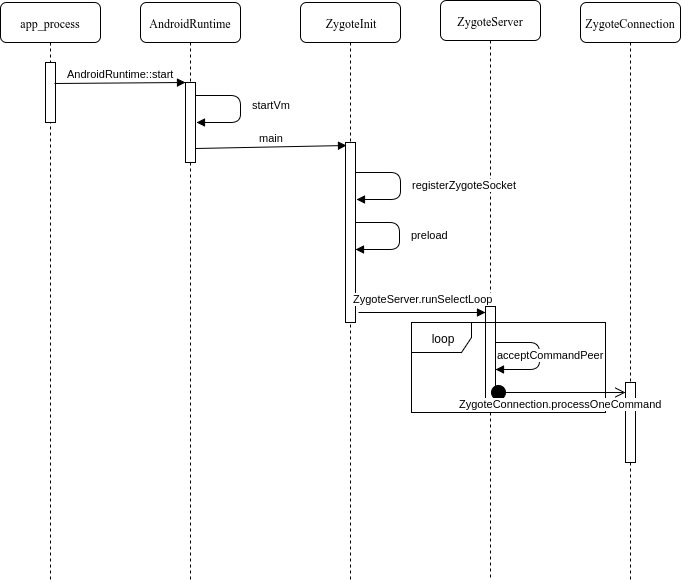
\includegraphics[width=\textwidth]{zygote_start.jpg}
	\caption{Zygote进程启动过程}
	\label{zygoteStart}
\end{figure}

首先系统会启动/system/bin目录下的本地程序app\_process, app\_process解析自身参数后若发现参数中有--zygote就会将进程名改为Zygote然后调用AndroidRuntime::start启动Android运行时环境, 并把入口类设置为com.android.internal.os.ZygoteInit\juhao 进入AndroidRuntime后, 会调用startVM启动ART虚拟机, 之后就会开始执行上述入口类ZygoteInit的main方法\juhao 该类的main方法中首先调用registerZygoteSocket注册一个socket用于之后从该socket接收创建应用进程的命令并执行, 然后会调用preload加载许多重要的类, 最后会调用ZygoteServer.runselectLoop进入一个死循环\juhao 至此, Zygote进程就启动完成了\juhao 在runselectLoop的死循环中, 其会调用acceptCommandPeer等待创建应用的命令, 接收到命令后调用ZygoteConnection.processOneCommand使用fork机制来创建新进程, 所以Zygote在启动后会一直执行runselectLoop直到关机\juhao

了解了Zygote进程的启动过程后, 下面是Android应用的启动过程\juhao Android应用是通过四大组件构成的, 这里通过启动一个Activity的过程来介绍应用的启动过程\juhao 图\ref{appStart}和\ref{appStart2}描述了启动一个没有运行的应用的过程(省略了一些不需要关心的调用)\juhao
\begin{figure}[ht]
	\centering
	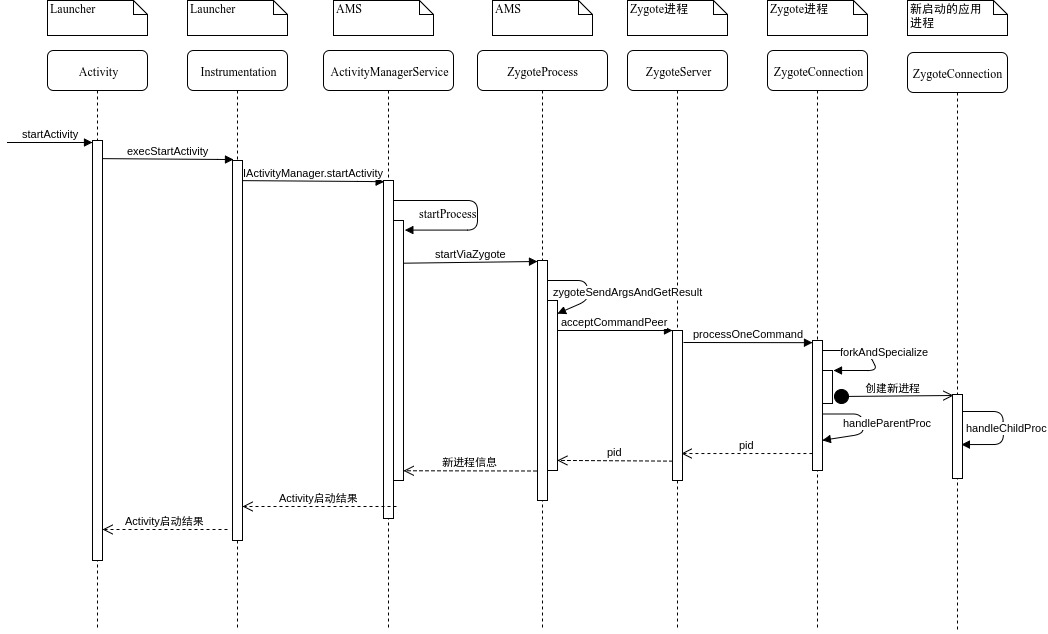
\includegraphics[width=\textwidth]{app_start.jpg}
	\caption{应用启动过程-1}
	\label{appStart}
\end{figure}

\begin{figure}[ht]
	\centering
	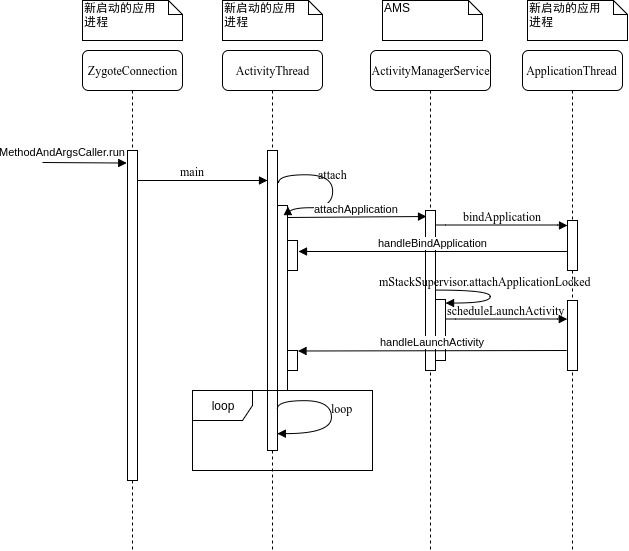
\includegraphics[width=\textwidth]{app_start2.jpg}
	\caption{应用启动过程-2}
	\label{appStart2}
\end{figure}
首先启动器调用Activity类的startActivity方法用于启动一个Activity, 该方法又会调用Instrumentation类的execStartActivity方法\juhao  execStartActivity通过Binder机制远程调用系统服务ActivityManagerService(AMS)的startActivity方法来创建Activity\juhao 由于应用还没有启动, AMS会调用startProcessLocked来创建新应用的进程, 该方法最终会调用ZygoteProcess类的zygoteSendArgsAndGetResult方法通过在介绍Zygote进程启动部分提到的socket来传递参数让Zygote进程生成一个新的应用进程\juhao Zygote进程接收到创建新进程的命令后执行forkAndSpecialize方法产生一个新的进程, 并把该进程pid返回给AMS\juhao 新创建的进程通过handleChildProc来做一些初始化操作, 比如关闭Zygote进程的socket, 之后会找到android.app.ActivityThread类并开始执行其main函数\juhao 这时候应用APK文件还没有被加载, 该进程还没有与具体的应用程序关联起来, 加载应用APK文件中的数据的操作通过ActivityThread类的attach方法完成\juhao ActivityThread类的main函数会调用本类的attach方法, 该方法又会通过Binder机制远程调用AMS中的attachApplication方法\juhao attachAppication方法完成新建应用的注册操作后会通过Binder机制远程调用新启动应用ActivityThread类中的ApplicationThread类的bindApplication方法\juhao ApplicationThread类是一个Binder类, 其bindApplication通过Handle机制调用ActivityThread类中的handleBindApplication方法完成应用的绑定与加载工作, 并创建Application实例\juhao bindApplication操作完成后, AMS会通过类似机制最终调用handlelaunchActivity完成Activity的启动, 至此, 应用就成功启动了\juhao 

\subsection{类的加载}
\label{classLoadA}
Android应用的类保存在dex文件里, 从dex文件加载类一般有3个过程:首先时加载dex文件, 之后加载类, 最后链接类\juhao 图\ref{classLoad}描述了使用Android系统的PathClassLoader加载一个类的过程\juhao 
\begin{figure}[ht]
	\centering
	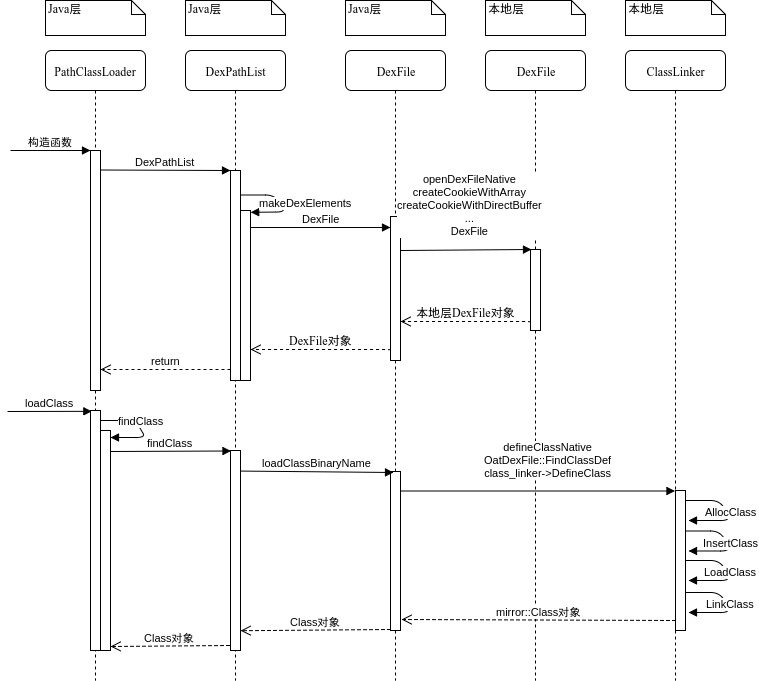
\includegraphics[width=\textwidth]{class_load.jpg}
	\caption{类的加载过程}
	\label{classLoad}
\end{figure}
PathClassLoader用于加载应用APK文件中包含的dex文件中的类\juhao PathClassLoader的构造函数通过其父类的构造函数调用了DexPathList的构造函数来加载应用的所有dex文件\juhao 在DexPathList的构造函数中, 其调用了makeDexElements来加载每一个dex文件\juhao makeDexElements又会调用DexFile类的构造函数来获取一个dex文件对象\juhao DexFile类的构造函数通过openDexFileNative等一系列JNI方法进入本地层调用相关函数将dex文件加载到内存中, 最后调用了本地层的DexFile类的构造函数完成对dex文件各字段的解析得到本地层的DexFile对象\juhao 该对象最后被传递给Java层的DexFile对象, 并记录在其mCookie成员变量中, 完成了dex文件的加载\juhao

当某个类需要被加载时, 会调用PathClassLoader的loadClass方法\juhao 在该类还未被加载过时, loadClass方法会调用findClass方法, findClass方法会接着调用记录着DexFile对象的DexPathList对象的findClass方法\juhao DexPathList对象的findClass方法会尝试遍历所有的DexFile对象, 并调用每一个DexFile对象的loadClassBinaryName对象来加载目标类, 直到在某个DexFile对象成功加载该类为止\juhao DexFile对象的loadClassBinaryName会通过defineClassNative这个JNI方法调用本地层的OatDexFile::FindClassDef方法找到该类在dex文件中的位置, 之后调用ClassLinker::DefineClass完成类的加载和链接工作, 并生成本地层的mirror::Class对象代表该类\juhao 通过该对象构造的Java层的Class对象最终会成为findClass的返回值, 这样一个类就完成了加载和链接, 可以被调用了\juhao 

\subsection{方法的执行}
\label{methodExecA}
为了提高运行效率ART虚拟机的运行机制一直在发生变化, 在Android8.1中, 应用的dex文件已经不会在安装时通过dex2oat全部编译而是在之后根据应用运行的情况按需编译, 同时JIT机制被再次启用, 并增加了对方法执行情况的统计用于在系统空闲时按需编译特定方法\juhao 因此, 一个非JNI方法有三种执行方式:第一种是通过解释器执行; 第二种是通过Just-In-Time(JIT)编译后的机器码执行; 第三种是通过Ahead Of Time(AOT)编译后的机器码执行\juhao 但总的说来, 方法的执行只有两种, 一种是解释执行字节码, 另一种是执行机器码\juhao 
所有执行机器码的方法, 都会调用Android源代码中的/art/runtime/ArtMethod.cc中的ArtMethod::Invoke函数来执行, 所有执行字节码的方法都会调用Android源代码中的/art/runtime/interpreter/interpreter.cc中的Execute函数来执行, 此外经过Java反射机制从Java层或者JNI反射机制从本地层调用Java方法会经过ArtMethod::Invoke来执行\juhao 图\ref{methodExec}和\ref{methodExec2}描述了ART几种不同的方法的执行流程\juhao 
\begin{figure}[ht]
	\centering
	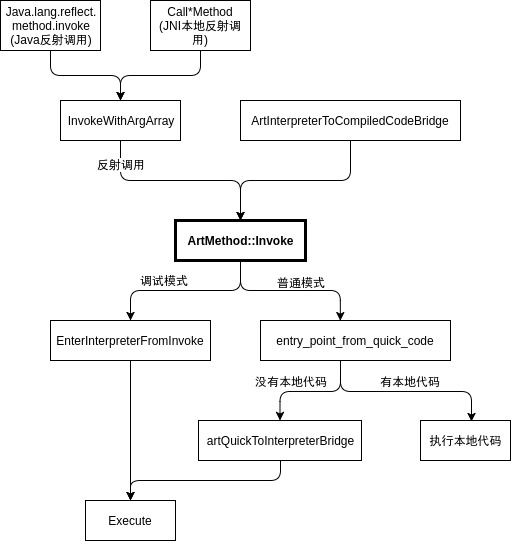
\includegraphics[width=\textwidth]{method_exec.jpg}
	\caption{ART中方法执行过程-1}
	\label{methodExec}
\end{figure}

\begin{figure}[ht]
	\centering
	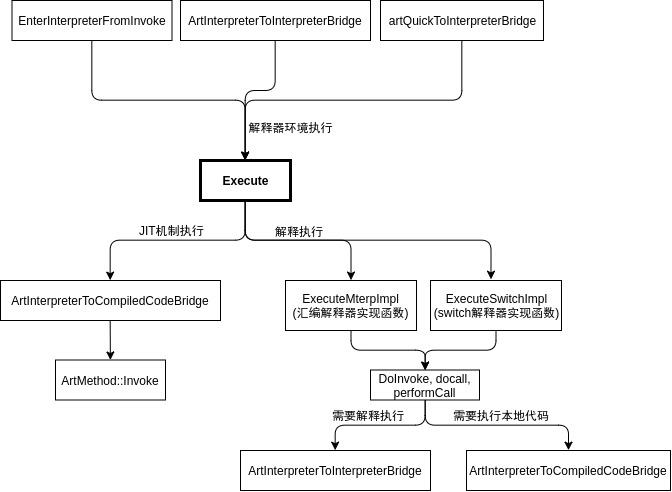
\includegraphics[width=\textwidth]{method_exec2.jpg}
	\caption{ART中方法执行过程-2}
	\label{methodExec2}
\end{figure}
图\ref{methodExec}主要描述了调用ArtMethod::Invoke来执行一个方法的情况\juhao ArtMethod::Invoke有两个入口, 第一个入口是使用Java反射(Java.lang.reflect.method.invoke方法)或JNI反射机制(Android源代码/art/runtime/reflection.cc中的一系列Call*Method函数)经过一系列调用后会调用InvokeWithArgArray\juhao InvokeWithArgArray会打包好方法的参数然后调用ArtMethod::Invoke来执行方法\juhao 该路径的调用的方法可能没有本地代码可以执行, 因此方法的入口点(entry\_point\_from\_quick\_code)可能会为artQuickToInterpreterBridge, 执行方法的入口后会进入解释模式并调用Execute来完成方法的执行; 第二个入口是解释模式执行的方法通过ArtInterpreterToCompiledCodeBridge调用有本地代码的方法, 此时若应用没有运行在调试模式, 会执行应用的本地代码\juhao 以上两个入口, 在应用处于调试模式时, 都会调用EnterInterpreterFromInvoke进入解释模式最后调用Execute执行目标方法\juhao 

图\ref{methodExec}主要描述了调用Execute来执行一个方法的情况\juhao Execute函数有三个入口, 第一个是EnterInterpreterFromInvoke, 用于从ArtMethod::Invoke中进入解释模式执行; 第二个是ArtInterpreterToInterpreterBridge, 用于解释执行的方法调用解释执行的方法; 第三个是artQuickToInterpreterBridge, 用于从本地代码中进入解释模式执行\juhao
在通过Execute函数解释执行方法时, 可能会启动JIT机制编译当前方法然后通过ArtInterpreterToCompiledCodeBridge进入ArtMethod::Invoke执行编译生成的本地代码, 而JIT机制没有启动时会调用解释器函数开始执行方法\juhao Android8.1系统中有两个不同实现方案的解释器函数:第一个是ExecuteMterpImpl, 该函数通过汇编代码实现, 效率很高, 但实现复杂, 不支持调试; 第二个是ExecuteSwitchImpl, 该函数通过switch语句实现, 支持单步调试, 实现也比较简单但运行效率很低, 只有在调试模式的情况下使用\juhao 解释器函数在执行到调用其他方法的字节码时, 会依次调用DoInvoke\dunhao DoCall\dunhao performCall\juhao performCall会根据方法的类型和是否处于调试模式来决定调用ArtInterpreterToInterpreterBridge以解释模式执行还是调用ArtInterpreterToCompiledCodeBridge执行方法的本地代码\juhao 


\section{Android动态分析相关技术和实现工具}
Android平台的动态分析同传统PC环境有相似之处, 即都是通过追踪应用软件的控制流和数据流实现对应用软件行为的揭示\juhao 但Android系统的多层次架构使得动态分析系统需要能够同时对本地层和Java层对应用的执行进行监控才能够获取到应用的完整行为\juhao 对各层次的监控, 常用的技术如下:

\subsection{Virtual Machine Introspection}
Virtual Machine Introspection(VMI)是一种实时监控虚拟机运行状态的技术\juhao 通过该技术, 能够实现在指令层面监控应用的运行, 因此也可以实现对系统调用, 本地函数调用的监控\juhao 并且由于监控代码运行于客户系统之外, 客户系统内被监控的应用无法检测到自己处于被监控状态, 因此是一种十分有效的监控应用运行的技术\juhao 对于Android平台的动态监控而言, 使用VMI技术无需修改Android源代码, 可以适应Android版本的变化, 但该技术的运用依赖于模拟器, 一般通过修改模拟器加入监控代码来实现, 但由于依赖模拟器, 容易受到应用对模拟器环境检测的影响\juhao Cooperdroid\upcite{copperdroid}、DroidScope\upcite{droidscope}使用了该技术来实现动态监控\juhao

\subsection{ptrace系统调用}
ptrace系统调用是Unix和一些类Unix系统中的一种系统调用\juhao 通过使用ptrace系统调用, 一个进程可以监控另外一个进程的执行, 读取和修改其内存和寄存器\juhao 具体来说, ptrace系统调用能够实现监控应用调用系统调用的情况, 能够实现指令单步执行和断点, 许多调试工具都依赖于ptrace系统调用实现, 如gdb, lldb, strace, ltrace等\juhao 由于ptrace系统调用能够实现单步执行, 通过ptrace系统调用也能实现在指令层面监控应用的执行\juhao 加上ptrace系统调用能够监控应用调用系统调用的情况, 通过ptrace系统调用可以实现对本地函数调用的监控\juhao 对于Android平台的动态监控而言, 使用ptrace系统调用也无需修改Android源代码, 可以适应Android版本的变化, 并且相比VMI技术, ptrace系统调用不依赖于模拟器, 可以运行于真机上, 但存在一些反ptrace跟踪的技术, 例如一个进程只能被一个进程跟踪, 所以应用可以跟踪自身, 从而防止被其他工具跟踪\juhao ptrace系统调用一般还会和hooking技术结合起来使用, 可以实现对目标函数的劫持和监控\juhao Crowdroid\upcite{crowdroid}\dunhao Glassbox\upcite{glassbox}和DroidTrace\upcite{droidtrace}使用了该技术来实现动态监控\juhao

\subsection{Application Instrumentation}
Application Instrumentation指通过修改需要监控的目标应用, 向其中插入监控代码实现监控应用执行的技术\juhao 对于Android平台而言, 该技术一般用于监控应用调用Java层API的情况, 具体来说, 通过反编译应用的dex文件得到smali代码, 搜索其中调用敏感API的代码, 将监控代码插入调用敏感API代码的周围, 再将修改后的smali代码编译重新打包成包含监控代码的应用, 这样在应用执行时就会执行监控代码, 输出监控信息\juhao 该技术不需要修改Android系统源代码, 但受到Android系统API变化的影响, 因此会在一定程度上受Android版本变化的影响\juhao 此外, 由于应用完整性校验以及加壳和混淆技术的广泛应用, 修改后的应用很可能无法运行, 并且一般无法从应用安装包获取到包含应用真实逻辑的dex文件, 因此该技术目前几乎已经失效\juhao APIMonitor\upcite{apimonitor}\dunhao Droidward\upcite{droidward}\dunhao ConDroid\upcite{condroid} 和Droidcat\upcite{droidcat} 使用了该技术实现动态监控\juhao

\subsection{DVM/ART Instrumentation}
\label{artInstr}
DVM/ART Instrumentation指通过修改Android系统的DVM或者ART运行时环境, 在关键的部分加入监控逻辑实现监控应用在Java层执行情况的技术\juhao 一般来说, 可以修改Android运行时环境中方法执行相关的函数来实现对应用执行的方法以及其参数和返回值的监控, 也可以修改Android运行时环境中的字节码解释器实现对Java层指令级别的监控, 在\ref{androidRuntime}节有关于Android运行时环境更详细的描述\juhao 该方法有些类似于上面提到的VMI技术, 在虚拟机层面监控虚拟机内部运行的应用, 在实现全面监控应用运行的同时也使得应用无法检测到自己处于受监控状态, 因此是监控应用Java层行为的一种十分有效的技术\juhao 并且该技术不依赖于模拟器, 利用其开发的动态监控系统可以运行于真机上, 不受应用检测模拟器机制的影响\juhao 但该技术的实现依赖于对
Android源代码的修改, 并且Android运行时环境在不同版本上变化较大, 特别是Android5.0之前和Android5.0之后Android运行时环境有DVM替换为了ART, 因此需要经常调整以适用于最新的Android版本\juhao DroidScope\upcite{droidscope}\dunhao Glassbox\upcite{glassbox}使用了该技术实现动态监控\juhao

\subsection{Hooking技术}
hooking技术是一类劫持函数调用的技术, 通过hooking技术, 我们可以获取目标函数的参数和返回值, 可以改变目标函数的行为从而实现对目标函数的监控\juhao 对于Android平台, hooking技术可以用于监控本地函数也可以用于监控Java方法, 其具体的实现方式有很多种, 例如针对本地函数有Procedure Link Table(PLT) hooking\dunhao inline hooking\dunhao Import Address Table(IAT) hooking; 针对Java方法有修改vtable, 修改ArtMethod对象的入口地址等\juhao hooking技术一般比较灵活, 结合一些动态代码追踪工具, 例如frida, 能够动态的调整监控目标\juhao 由于ptrace系统调用能够修改被追踪进程的内存, linux系统的hooking技术一般会利用ptrace系统调用实现\juhao ARTdroid\upcite{artdroid}和REAPER\upcite{reaper}使用了该技术实现动态监控\juhao

\subsection{Frida}
\label{frida}
Frida\upcite{frida}是一个著名的开源跨平台动态代码追踪工具\juhao 该工具支持几乎所有常见的桌面或者移动操作系统, 并且提供了Javascript API来实现简单快速的开发\juhao 利用该工具的Javascript API, 可以实现劫持本地或者Java层的函数, 调用本地函数, 读写内存, 操作文件和socket, 修改指令等许多操作\juhao 但Frida框架在Andriod系统下存在一些兼容性问题, 容易导致应用崩溃\juhao 

\subsection{Xposed}
 Xposed\upcite{xposed} 是一个著名的Android平台的开源动态代码劫持框架\juhao
 Xposed框架可以在不修改应用APK文件的情况下劫持应用的Java方法从而执行一些操作从而改变应用的行为\juhao Xposed框架通过使用修改后的app\_process程序替换Android系统中/system/bin/app\_process程序来实现对Zygote进程的控制,并在启动时加载XposedBridge.jar提供从Java层调用Xposed框架的接口\juhao 根据\ref{appStartA}节介绍的Zygote进程与应用启动的关系, 可以看到应用会保留Zygote进程中加载的所有内容, 因此控制了Zygote进程就实现了对所有应用进程的控制\juhao Xposed框架提供了劫持Java方法的API
但不支持对本地函数劫持\juhao  Inspeckage\upcite{inspeckage}\dunhao InsightDroid\upcite{chinese1} 文献\cite{chinese2}中的系统使用该技术实现了动态监控\juhao 

\subsection{Valgrind}
Valgrind\upcite{valgrind}是一个用于构建动态分析工具的开源代码追踪框架, 可以被编译运行在许多类Unix系统中\juhao Android系统基于Linux构建, 因此利用Valgrind来构建动态分析系统\juhao Malton\upcite{malton}\dunhao PackerGrind\upcite{packergrind}使用了该技术来实现动态监控\juhao 

\section{Android应用保护技术}
为保护知识产权, 防止逆向分析, 许多Android应用都采用了加固技术来保护自己的代码, 目前常用的技术包括完整性校验\upcite{androidsecure}\dunhao 名称混淆\dunhao 方法执行混淆\upcite{tiro}\dunhao dex文件动态加载\upcite{packergrind}\dunhao dex文件动态修改\upcite{packergrind}\dunhao 类动态加载\upcite{packergrind}\dunhao 方法本地实现\upcite{packergrind}\dunhao 模拟器检测\upcite{emdetection}\dunhao 反调试\upcite{packergrind} 等\juhao

\paragraph*{完整性校验}
该技术为应用在运行具体的业务逻辑前先对自身的代码文件, 资源文件等文件计算校验值, 然后把校验值与应用未经过修改时的校验值进行比较, 如果相同则表示应用没有被修改, 可以运行; 如果不同则表示应用被篡改, 停止执行\juhao 完整性校验可以只在应用启动时执行,但容易被绕过, 也可以在应用内随机执行, 极大地增加绕过的难度\juhao 

\paragraph*{名称混淆}
该技术即在应用发布时按照一定的规则将开发应用时定义的有意义的类名\dunhao 方法名\dunhao 和变量名替换称无意义的字符, 从而增加了逆向分析方法用途的难度\juhao

\paragraph*{方法执行混淆}
该技术通过hooking技术使用将一个方法的代码用另外一个方法替换从而使得动态监控系统记录的方法调用和实际的方法调用不同, 因此能够隐藏应用行为, 极大地增加了动态分析的难度\juhao

\paragraph*{dex文件动态加载}
该技术通过先将包含应用真实逻辑的dex文件加密, 在应用运行时再调用解密代码释放dex文件并动态加载来实现隐藏包含应用真实逻辑的dex文件\juhao 该技术用于对抗静态分析十分有效, 可以使得静态分析无法获取到应用的真实逻辑\juhao

\paragraph*{dex文件动态修改}
该技术为dex文件动态加载技术的改进\juhao 采用该技术时, 加载到内存的dex文件并不完全解密, 而是在具体的方法调用前修改方法对应dex文件中的部分为方法的真正指令, 在方法执行后又抹去对应指令\juhao 该技术用于对抗一些Android平台的脱壳工具, 使其无法得到完整的dex文件\juhao

\paragraph*{类动态加载}
该技术把类方法的字节码分散到多个dex文件中, 在某个类被调用时动态的解密对应的dex文件来加载被调用的类, 从而极大地增加了脱壳工具获取包含应用真实逻辑的dex文件的难度\juhao

\paragraph*{方法本地实现}
该技术将某些方法替换成本地方法, 使用本地指令实现方法的内容, 从而加大了分析方法用途的难度\juhao 有些应用加固工具还结合了Virtual Machine Protection(VMP)技术, 将原始指令转换成自己的私有指令集并通过私有虚拟机执行, 进一步增加了分析方法内容的难度\juhao

\paragraph*{模拟器检测}
该技术使用了许多Android模拟器的特征来识别应用的运行环境是否为模拟器, 例如许多模拟器的International Mobile Equipment Identity(IMEI)为全0\juhao 由于许多动态分析工具依赖于模拟器, 所以一旦识别出当前运行在模拟器环境, 应用就可以退出或者表现出一些不同于真机上的行为, 从而阻碍动态分析\juhao

\paragraph*{反调试}
该技术通过多种方式检测应用是否处于被调试状态, 并阻止对应用的调试\juhao 例如, 应用通过调用ptrace追踪自身从而避免被其他监控进程追踪; 应用通过搜索内存中某些著名调试工具的名称, 如strace, ltrace, valgrind等来确定自身是否被调试; 应用hook自身的某些函数,如open, wrtie等来阻止自己的数据被调试工具输出\juhao 反调试技术给真机上的动态分析系统带来了较大的障碍而基于模拟器的动态分析系统可以把监控功能部署在Android系统的外部, 使得应用无法检测到监控工具的存在从而避免反调试技术的影响\juhao 




